\subsection{Joint vs Disjoint}\label{sec:joint-vs-disjoint}
We have discuss about joint and disjoint solutions, in the following section we want to compare these solutions in the optimal form with eachother.
For this comparison we use two different topology to have better insights and fair results.
We have changed number chains in each step and these chains are generated randomly with configuration mentioned in \ref{tlb:chain-configuration}.

\begin{table}[H]
  \caption{Chain Configuration}
  \label{tbl:chain-configuration}
  \centering
  \begin{tabular}{ll}
    \toprule
    Property & Value \\
    \midrule
    Length & $[4,7)$ \\
    Per Instance Cost & 100\$ \\
    Bandwidth & 250bps \\
  \end{tabular}
\end{table}

\subsubsection{FatTree}
Here we will use FatTree topology with k equals to 6. Each result is baed on 15 runs in the CPLEX with the limited time and optimality gap.
As you can see results confirm our hypothesis that joint solutions makes better revenues.

\begin{table}[H]
    \caption{Revenues from Joint and Disjoint Solutions on FatTree Topology with k equals to 6}
    \label{tbl:joint-vs-disjoin-fattree}
    \medskip
    \centering
    \begin{tabular}{lrrr}
        \toprule
        {} &         joint &      disjoint &  nchains \\
        \midrule
        0  &   4453.333333 &   1913.333333 &       10 \\
        1  &   6586.666667 &   1000.000000 &       15 \\
        2  &   8886.666667 &   1593.333333 &       20 \\
        3  &  11133.333333 &   3266.666667 &       25 \\
        4  &  13326.666667 &   7906.666667 &       30 \\
        5  &  15466.666667 &  13073.333333 &       35 \\
        6  &  17973.333333 &  14686.666667 &       40 \\
        7  &  20146.666667 &  17553.333333 &       45 \\
        8  &  22440.000000 &  15633.333333 &       50 \\
        9  &  24446.666667 &  14613.333333 &       55 \\
        10 &  26940.000000 &  14713.333333 &       60 \\
        11 &  29313.333333 &  18886.666667 &       65 \\
        12 &  31486.666667 &  16313.333333 &       70 \\
        13 &  33713.333333 &  17340.000000 &       75 \\
        14 &  36253.333333 &  19553.333333 &       80 \\
        15 &  37846.666667 &  18540.000000 &       85 \\
        16 &  40500.000000 &  23360.000000 &       90 \\
        \bottomrule
    \end{tabular}
\end{table}

\begin{figure}[H]
    \centering
    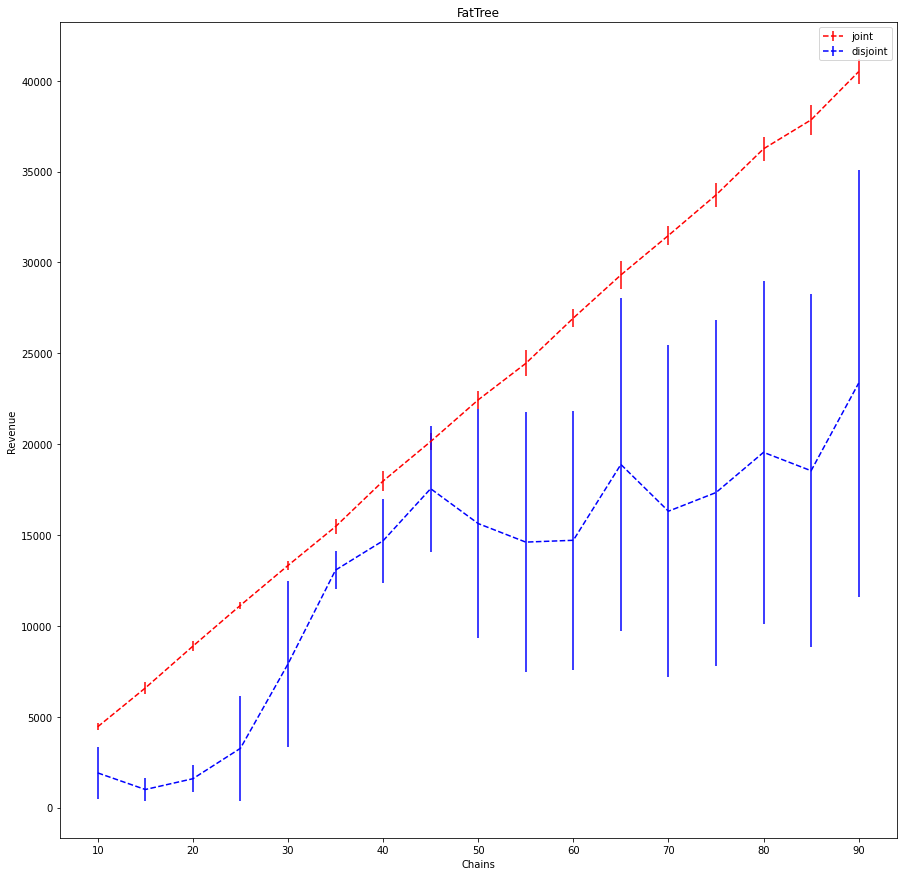
\includegraphics[height=350pt]{plots/joint-vs-disjoint-fattree.png}
    \caption{Revenues from Joint and Disjoint Solutions on FatTree Topology with k equals to 6}
    \label{fig:joint-vs-disjoint-fattree}
\end{figure}

\subsection{USNet}
Here we will use USNet topology with 3 to 4 nodes attached to each of its points.
As you can see the results show joint and disjoint solutions on this setup work equally because there is no specific
management requirement and topology can handle all chains.

\begin{table}[H]
    \caption{Revenues from Joint and Disjoint Solutions on USNet Topology}
    \label{tbl:joint-vs-disjoin-usnet-1}
    \medskip
    \centering
    \begin{tabular}{lrrr}
        \toprule
        {} &    joint &  disjoint &  nchains \\
        \midrule
        0 &  23000.0 &   23010.0 &       50 \\
        1 &  34180.0 &   34260.0 &       75 \\
        2 &  45430.0 &   45560.0 &      100 \\
        3 &  57180.0 &   57380.0 &      125 \\
        4 &  68750.0 &   69360.0 &      150 \\
        \bottomrule
    \end{tabular}
\end{table}

\begin{figure}[H]
    \centering
    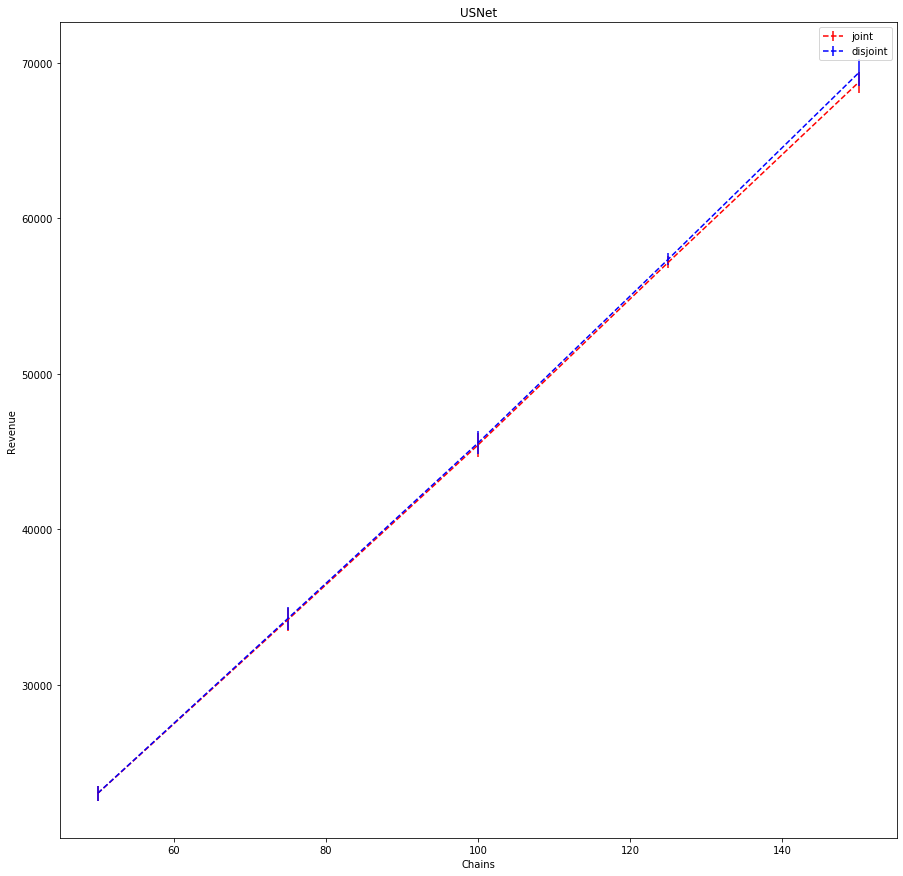
\includegraphics[height=350pt]{plots/joint-vs-disjoint-usnet-1.png}
    \caption{Revenues from Joint and Disjoint Solutions on USNet Topology}
    \label{fig:joint-vs-disjoint-usnet-1}
\end{figure}

But we continue by adding an specific management constriant which is the distance between manager and chain's nodes must be less than equal to 4 and then the difference increases.

\begin{table}[H]
    \caption{Revenues from Joint and Disjoint Solutions on USNet Topology with Managemnt Constraint}
    \label{tbl:joint-vs-disjoin-usnet-2}
    \medskip
    \centering
    \begin{tabular}{lrrr}
        \toprule
        {} &         joint &      disjoint &  nchains \\
        \midrule
        0  &   4473.333333 &   1420.000000 &       10 \\
        1  &   6926.666667 &   2733.333333 &       15 \\
        2  &   8940.000000 &   3533.333333 &       20 \\
        3  &  11133.333333 &   4833.333333 &       25 \\
        4  &  13313.333333 &   9020.000000 &       30 \\
        5  &  15486.666667 &  14693.333333 &       35 \\
        6  &  17913.333333 &  15433.333333 &       40 \\
        7  &  19813.333333 &  17586.666667 &       45 \\
        8  &  22213.333333 &  21020.000000 &       50 \\
        9  &  24113.333333 &  21866.666667 &       55 \\
        10 &  26640.000000 &  24546.666667 &       60 \\
        11 &  28833.333333 &  25760.000000 &       65 \\
        12 &  31360.000000 &  29420.000000 &       70 \\
        13 &  33140.000000 &  29660.000000 &       75 \\
        14 &  35686.666667 &  33320.000000 &       80 \\
        15 &  37600.000000 &  34986.666667 &       85 \\
        16 &  39840.000000 &  37473.333333 &       90 \\
        \bottomrule
    \end{tabular}
\end{table}

\begin{figure}[H]
    \centering
    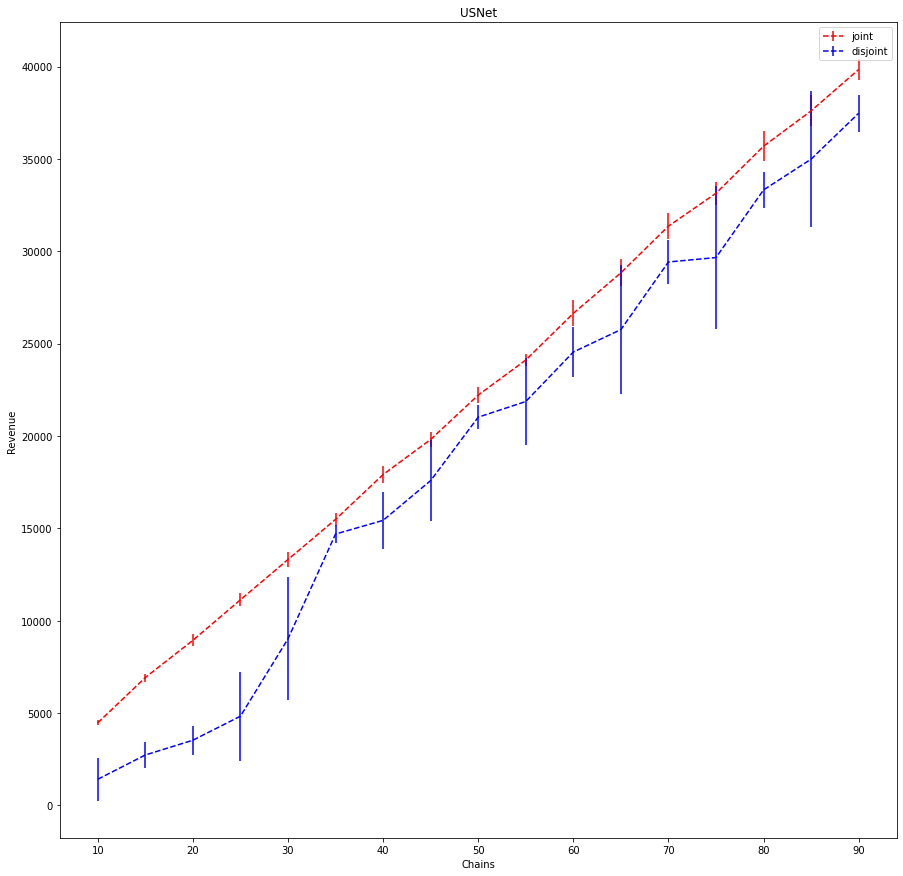
\includegraphics[height=350pt]{plots/joint-vs-disjoint-usnet-2.png}
    \caption{Revenues from Joint and Disjoint Solutions on USNet Topology with Management Constraint}
    \label{fig:joint-vs-disjoint-usnet-2}
\end{figure}
